%%%
% Manual Layout Functions
%%%

\section{Hilfefunktionen für manuelles Layout}
\label{sec:manual-layout}

In Anwendungen zum Erstellen von Diagrammen wie z.B. Vektorgrafik-Software, Präsentationsprogramme oder CASE-Tools wird in der Regel ausschließlich das manuelle Layout unterstützt. Das bedeutet, dass der Nutzer die Diagrammbestandteile im Canvas frei verschieben kann und somit einen großen Einfluss auf das resultierende Layout des Diagramms hat. Um einige manuellen Schritte während der Erstellung eines Diagramms zu sparen, bieten die Anwendungen eine Reihe an Funktionen an, mit deren Hilfe sich das Layout besser gestalten lässt. Diese werden im Detail in diesem Abschnitt beschrieben.

% TODO: Temporäre Layout-Funktionen, es werden keine Regeln gebildet

% TODO: Beschreibung der Apps (OmniGraffle, Keynote, ConceptDraw und Visual Paradigm), an den die Funktionen gezeigt werden
% OmniGraffle ("die folgenden Erkenntnisse wurden durch die Arbeit mit OmniGraffle 5 gewonnen")

\subsection{Raster}
\label{sec:grid}

Viele Visualisierungsprogramme (unter anderem alle 4 erwähnten) unterstützen die Aufteilung des Canvas in einen gleichmäßigen Raster, der durch Rasterlinien dargestellt wird. Diese Linien können zum Ausrichten von Objekten im Canvas verwendet werden. Dies ist vor allem für die Diagramme nützlich, in der die Größen der Objekte eine wichtige Rolle spielen wie z.B. Grundrisse \cite{08OmniGraffle, Olsen10OmniGraffle, 11Keynote, 14Visual}.

\begin{figure}[hbt]
    \centering
    % TODO: Neuer Screenshot mit aktiviertem Snap-to-Grid
    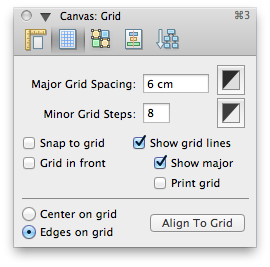
\includegraphics[width=0.5\textwidth]{resources/omnigraffle-grid-settings.png}
    \caption{Informationsfenster zur Einstellung des Rasters in OmniGraffle}
    \label{fig:omnigraffle-grid-settings}
\end{figure}

In Abbildung \ref{fig:omnigraffle-grid-settings} wird ein Informationsfenster aus OmniGraffle dargestellt, in dem die Einstellungen des Rasters für das bearbeitete Diagramm vorgenommen werden können. Neben der Einstellung der Rastergröße können an dieser Stelle die Rasterlinien ein- und ausgeblendet, die Funktion \textit{Snap-to-Grid} aktiviert und die Funktion \textit{Ausrichten im Raster} ausgeführt werden \cite{08OmniGraffle}.

\subsubsection{Snap-to-Grid}

Die reguläre Verschiebungsoperation von Objekten im Diagramm funktioniert in der Regel wie folgt: Der Nutzer wählt mit dem Mauszeiger ein Objekt aus und schiebt das Objekt mit gedrückter Maustaste auf seine neue Position. Wenn die Funktion \textit{Snap-to-Grid} nicht aktiviert ist, kann die Zielposition beliebig sein. Während der Verschiebung wird die Position des Objekts kontinuierlich angepasst, so dass der Nutzer einen visuellen Feedback bekommt. Dieser Vorgang ist in Abbildung X dargestellt.

% TODO: Abbildung: Verschiebungsoperation mit nicht aktivierter Funktion \textit{Snap-to-Grid} in OmniGraffle

Wenn die Funktion \textit{Snap-to-Grid} nun aktiviert ist, wird im Unterschied zu dem vorigen Vorgang die Zielposition so eingeschränkt, dass das verschobene Objekt an die Rasterlinien ausgerichtet wird. Der Mauszeiger kann dabei frei positioniert werden, das Objekt nimmt aber immer die nächste ausgerichtete Position an. Dieser Vorgang ist in Abbildung X dargestellt.

% TODO: Abbildung: Verschiebungsoperation mit aktivierter Funktion \textit{Snap-to-Grid} in OmniGraffle

Neben der Verschiebungsoperation wird auch die Operation der Größenänderung eingeschränkt, indem das manipulierte Objekt nur so eine Größe annehmen kann, die die Ausrichtung an die Rasterlinien nicht verletzt.

\subsubsection{Ausrichten im Raster}

Das Ausrichten an die Rasterlinien kann auch nachträglich bewirkt werden. Dies passiert durch die Auswahl des zu ausgerichteten Objekts und dem Ausführen der Funktion \textit{Ausrichten im Raster}. Danach wird die Position und Größe des Objekts so angepasst, dass das Objekt an die Rasterlinien ausgerichtet wird (siehe Abbildung X).  

% TODO: Abbildung: Funktion \textit{Ausrichten im Raster} in OmniGraffle

\subsection{Ausrichten und Verteilen von Objekten in Relation zueinander}

Ähnlich wie der Raster (Abschnitt \ref{sec:grid}) werden die Funktionen zum Ausrichten und Verteilen von ausgewählten Objekten häufig in Visualisierungsprogrammen eingesetzt. Sie funktionieren wie folgt: Der Nutzer wählt im Diagramm Objekte aus, an die die Funktion angewendet werden soll. Nachher wählt er eine konkrete Form der Funktion aus, die anschließend auf die ausgewählten Objekt angewendet wird \cite{11Keynote}.

\subsubsection{Ausrichten}

Die ausgewählten Objekte können in Relation zueinander ausgerichtet werden. Dafür muss nach der Auswahl von mindestens 2 Objekten die Form der Ausrichtung angegeben werden. Die Objekte können entweder vertikal (linke Kanten, Mittelpunkte oder rechte Kanten) oder horizontal (obere Kanten, Mittelpunkte oder untere Kanten) ausgerichtet werden. Nach dem Ausführen dieser Funktion werden die Positionen der ausgewählten Objekte so angepasst, dass die gewünschte Ausrichtung erfüllt ist \cite{11Keynote, 08OmniGraffle}. Ein Beispiel ist in Abbildung X zu finden.

% TODO: Abbildung: Anwendung der horizontalen Ausrichtung in Keynote

\subsubsection{Verteilen}

Wenn mindestens 3 Objekte ausgewählt werden, kann die Funktion zum gleichmäßigen Verteilen der Objekte angewendet werden. Dabei wird die Position der äußeren Objekte fixiert und die Position von umschlossenen Objekten wird so angepasst, dass die vertikalen bzw. horizontalen Abstände zwischen den Objekten gleich sind \cite{11Keynote}.

% TODO: Abbildung: Anwendung der horizontalen Verteilung in Keynote

\subsection{Smart Guides}
\label{subsec:smart-guides}

Eine sehr hilfreiche Funktion, die in den meisten Grafik- und Präsentationsprogrammen unterstützt wird, sind Hilfslinien für Ausrichtung und relative Positionierung (engl. \textit{Smart Guides}) \cite{11Keynote}. Wenn diese Funktion aktiviert ist, werden während der Manipulation des ausgewählten Objekts farbige Linien im Canvas eingeblendet. Diese Linien geben dem Nutzer einen visuellen Feedback zur geeigneten Ausrichtung des manipulierten Objekts relativ zu anderen Objekten im Diagramm. Außerdem wird ähnlich wie bei der Funktion \textit{Snap-to-Grid} die freie Manipulation eingeschränkt, das in der Regel zu besseren Layout-Ergebnissen führt. Die Hilfslinien werden nach der Beendigung der Operation wieder ausgeblendet und die Position bzw. Größe des manipulierten Objektes wird angepasst. Genauso wie auch bei allen anderen Hilfsfunktionen für das manuelle Layout handelt es sich bei den Hilfslinien um eine temporäre Layout-Funktion. Somit wird die Ausrichtung der Objekte nur in den Eigenschaften der Objekte (Position und Größe) ausgedrückt und es wird keine explizite Regel erstellt.

\subsubsection{Hilfslinien zur Ausrichtung (Alignment Guides)}

Die erste Art der Hilfslinien ist für die Ausrichtung des verschobenen Objekts an die Kanten bzw. Mittelachsen von anderen Objekten in Diagram nützlich. Die Linien werden während der Verschiebungsoperation eingeblendet, wenn das verschobene Objekt an ein anderes Objekt ausgerichtet wird \cite{11Keynote}. In Abbildung X wird ein Beispiel der Hilfslinien zur Ausrichtung der unteren Kanten von 2 Objekten während der Verschiebungsoperation gezeigt.

% TODO: Abbildung: Hilfslinien zur Ausrichtung während der Verschiebungsoperation in OmniGraffle

Aus der Abbildung X kann man entnehmen, dass sich um die untere Kante des inaktiven Objekts ein Bereich bildet, in dem das verschobene Objekt auf die ausgerichtete Position hinspringt. Dies passiert wenn die Gerade, die durch eine Kante oder Mittelachse des verschobenen Objektes gebildet wird, in der Nähe einer anderen Geraden, die durch eine Kante oder Mittelachse eines anderen Objektes im Diagramm gebildet wird, befindet und der Abstand unter einer bestimmten Schwelle liegt. Dieses Verhalten wird in Abbildung X visualisiert.

% TODO: Abbildung: Visualisierung des Bereichs für die Hilfslinien zur Ausrichtung

Solche Bereiche werden für alle Kanten und Mittelachsen von nicht ausgewählten Objekten in der horizontalen und vertikalen Richtung identifiziert. Wenn der Nutzer ein Objekt verschiebt und eine der Kanten oder die Mittelachse des verschobenen Objekts sich in einem der Bereichen befindet, wird das verschobene Objekt an die ausgerichtete Position positioniert, ohne den Mauszeiger zu beeinflussen. Das kann auch gleichzeitig für die horizontale und vertikale Richtung der Fall sein. Somit kann z.B. ein Objekt in einem anderen Objekt zentriert werden (siehe Abbildung \ref{fig:omnigraffle-alignment-guides-centering}).

\begin{figure}[hbt]
    \centering
    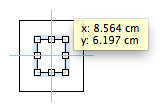
\includegraphics{resources/omnigraffle-alignment-guides-centering.png}
    \caption{Ausrichten eines Objekts in einem anderen Objekt mit Hilfe von einer horizontalen und einer vertikalen Hilfslinie zur Ausrichtung in OmniGraffle}
    \label{fig:omnigraffle-alignment-guides-centering}
\end{figure}

Eine Veranschaulichung dieser Funktion bietet in Form einer JavaScript-Anwendung\footnote{\url{http://mrflix.github.io/Alignment-Guides/}} das Open-Source Projekt \textit{Alignment-Guides}\footnote{\url{https://github.com/mrflix/Alignment-Guides}}.

\subsubsection{Abstandshilfslinien (Distance Guides)}

Die zweite Art der Hilfslinien dient dazu, die Abstände zwischen 3 Objekten in einer horizontalen oder vertikalen Reihe gleich zu halten. Während der Verschiebung eines der 3 Objekten wird ein Bereich gebildet, in dem das Objekt zu der Position hinspringt, in der die Abstände zwischen den einzelnen Objektpaaren gleich sind. Zusätzlich zu den Hilfslinien wird auch der Abstand eingeblendet \cite{11Keynote, Olsen10OmniGraffle}.

\begin{figure}[hbt]
    \centering
    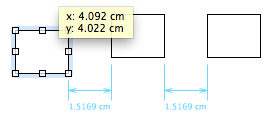
\includegraphics{resources/omnigraffle-distance-guides.png}
    \caption{Abstandshilflinien in OmniGraffle}
    \label{fig:omnigraffle-distance-guides}
\end{figure}

\subsubsection{Größenhilfslinien (Sizing Guides)}

Im Unterschied zu den zwei vorigen Arten der Hilfslinien wird die letzte Art durch die Operation der Größenänderung eines Objektes hervorgerufen. Wenn sich die Größe des manipulierten Objekts der Größe eines anderen Objekts im Diagramm nähert und die Differenz unter einer bestimmten Grenze liegt, wird die Größe des anderen Objekts übernommen. Dies funktioniert getrennt für die Breite und Höhe (siehe Abbildung \ref{fig:omnigraffle-sizing-guides}).

\begin{figure}[hbt]
    \centering
    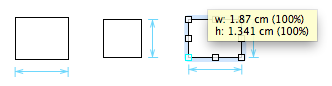
\includegraphics{resources/omnigraffle-sizing-guides.png}
    \caption{Größenhilfslinien in OmniGraffle}
    \label{fig:omnigraffle-sizing-guides}
\end{figure}

\subsection{Manuelle Hilfslinien}

Weiterhin bieten OmniGraffle und Keynote die Funktion der Erstellung von manuellen Hilfslinien an \cite{08OmniGraffle, 11Keynote}. Diese Funktion ist sehr ähnlich zu \textit{Smart Guides}, unterscheidet sich aber wie folgt:

\begin{itemize}
    \item Die Hilfslinien werden vom Nutzer manuell platziert - entweder horizontal oder vertikal.
    \item Die Hilfslinien sind global für das gesamte Diagramm und damit nicht relativ zu einem anderen Objekt im Diagramm.
    \item Die Hilfslinien sind permanent sichtbar, auch wenn keine Verschiebungsoperation stattfindet.\footnote{Die Anzeige der manuellen Hilfslinien kann sowohl in OmniGraffle als auch in Keynote global aus- und eingeschaltet werden.}
\end{itemize}

Die Gemeinsamkeit besteht darin, dass das Ausrichten an die Hilfslinien identisch wie bei den \textit{Smart Guides} funktioniert (siehe Abschnitt \ref{subsec:smart-guides}). Ein Bespiel der manuellen Hilfslinie in OmniGraffle wird in Abbildung \ref{fig:omnigraffle-manual-guides} dargestellt.

\begin{figure}[hbt]
    \centering
    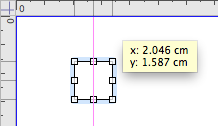
\includegraphics{resources/omnigraffle-manual-guides.png}
    \caption{Beispiel einer manuellen Hilfslinie in OmniGraffle}
    \label{fig:omnigraffle-manual-guides}
\end{figure}

\subsection{Gleiche Größe der Objekte}

Sehr trivial, aber dennoch nützlich ist die Funktion der Einstellung von gleichen Größen für ausgewählte Objekte. Nach der Auswahl von 2 oder mehreren Objekten im Diagramm hat der Nutzer die Möglichkeit, die Breite, die Höhe oder beide Dimensionen gleichzeitig auf die Werte des zuerst ausgewählten Objektes zu setzen (siehe Abbildung \ref{fig:omnigraffle-make-same-size}). Diese Funktion wird in OmniGraffle unterstützt \cite{Olsen10OmniGraffle}.

\begin{figure}[hbt]
    \centering
    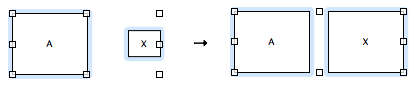
\includegraphics{resources/omnigraffle-make-same-size.png}
    \caption{Anwendung der Funktion zur Einstellung von gleichen Größen in OmniGraffle}
    \label{fig:omnigraffle-make-same-size}
\end{figure}

\subsection{Verknüpfungspunkte für Verbindungen}

% TODO: Verweis auf die Grundlagen (graph-basierte Diagramme)

Die bisher diskutierten Hilfsfunktionen haben sich ausschließlich mit der Positionierung und Bestimmung der Größe der Objekte auseinandergesetzt. Für die graph-basierten Diagramme sind neben der Knoten auch Kanten von Interesse, die in der Regel durch Verbindungslinien dargestellt werden. Wenn 2 Objekte mit einer Verbindungslinie verbunden werden, bleiben sie auch dann verbunden, wenn sich die Position oder Größe der Objekte ändert \cite{11Keynote}. In vielen Programmen (unter anderem in Keynote und OmniGraffle) werden die Verknüpfungspunkte der Verbindungslinie standardmäßig an die Stellen positioniert, an den eine gedachte Strecke, die die Mittelpunkte beider Objekte verbindet, die Kanten der Objekte schneidet (siehe Abbildung \ref{fig:omnigraffle-default-connection-points}) \cite{08OmniGraffle}.

\begin{figure}[hbt]
    \centering
    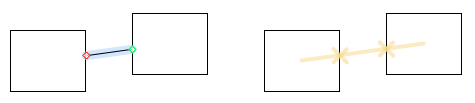
\includegraphics{resources/omnigraffle-default-connection-points.png}
    \caption{Verknüpfungspunkte einer Verbindung in OmniGraffle (links) mit Darstellung der Berechnung (rechts)}
    \label{fig:omnigraffle-default-connection-points}
\end{figure}

OmniGraffle bietet die Möglichkeit, mit Hilfe des Magnetwerkzeugs manuell die Verknüpfungspunkte zu definieren. Dies funktioniert auf zwei verschiedene Arten. Entweder kann der Nutzer die Verknüpfungspunkte beliebig in dem Objekt positionieren oder er wählt eine vordefinierte Anordnung aus. Dazu gehören u.a. die gleichmäßige Verteilung einer festen Anzahl an Verknüpfungspunkten entlang allen Kanten oder die Positionierung eines Verknüpfungspunktes an jedem Eckpunkt. Ein Beispiel der Darstellung von Verknüpfungspunkten ist in Abbildung \ref{fig:omnigraffle-magnets-example} zu finden.

\begin{figure}[hbt]
    \centering
    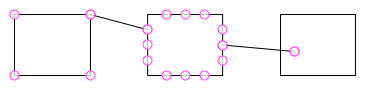
\includegraphics{resources/omnigraffle-magnets-example.png}
    \caption{Beispiel der manuellen Verknüpfungspunkte in OmniGraffle: Magnete an den Eckpunkten (links), 3 Magnete pro Kante (Mitte), ein manuell positionierter Magnet (rechts)}
    \label{fig:omnigraffle-magnets-example}
\end{figure}

Sobald mindestens ein Magnet dem Objekt hinzugefügt wurde, wird nicht mehr der Verknüpfungspunkt mit Hilfe des Mittelpunktes berechnet wie oben beschrieben, sondern die Verbindungslinie wird immer von dem nächsten Verknüpfungspunkt angezogen (siehe Abbildung \ref{fig:omnigraffle-magnets-example}). Alternativ kann der Nutzer ein Ende der Verbindungslinie an einen konkreten Verknüpfungspunkt binden. In dem Fall bleibt die Verbindungslinie an den gewählten Verknüpfungspunkt gebunden, auch wenn ein anderer Verknüpfungspunkt näher ist.

\subsection{Zusammenfassung der Eigenschaften}

% Mit dieser Funktion (manuelle Hilfslinien) ist der Nutzer in der Lage das Layout präziser zu steuern.
